\documentclass[11pt, oneside]{article}
\usepackage{geometry}
\geometry{letterpaper}
\usepackage[francais]{babel}
\usepackage[utf8]{inputenc}
\usepackage{graphicx}
\usepackage{float}
\usepackage{etex,mathtools}
\usepackage{amssymb}
\usepackage{enumitem}
\usepackage{amsmath}
\usepackage{caption}
\usepackage{listings}
\usepackage{array}
\usepackage[]{algorithm2e}
\title{Rapport de projet, Sparse wavelet}
\author{Louis Thiry, Alexandre Saint-Dizier}
\begin{document}

\maketitle

%Je suis plutot chaud pour garder le rapport en 2 partie : etude des donnes et solutions proposee.
%Le fichier data_transform rentre selon moi dans la premiere partie, et review dans la deuxieme.

\section*{Introduction}

Pendant la présentation des projets par les entreprises, nous avons été séduits par le projet de prédiction de la qualité de l'air à l'échelle de la rue de Plume Labs.
En effet, le problème en question est un problème de physique, et l'on peut espérer s'inspirer de son intuition pour proposer des solutions.
De plus, l'application, la prédiction de la pollution à l'echelle de la rue, est intéressante et utile.

Cependant, quand nous avons commencé à étudier les données, nous nous sommmes rendus compte qu'un bon nombre de paramètres relevant de la physique du problème étaient exclus dans les données fournies, ce qui empêchait d'avoir une approche physique et qui remettait sérieusement en cause l'ambition affichée: prédire la qualité de l'air à l'échelle de la rue.
Nous avons contacté Plume Labs pour en savoir plus, et ils nous ont répondu que cela était volontaire, le but réel du projet étant de "prédire la pollution à des points précis à partir d'informations statiques sur ces points et d'informations structurelles extraites sur les séries temporelles".

C'est donc à ce problème que nous nous sommes attaqués, problème très intéressant, mais aussi très général pour lequel on voit mal comment on peut obtenir des prédictions précises.



\section{Les données à notre disposition}

Les données du problème concernent les contentrations de trois types de polluants ($NO_2$, $PM_{10}$, $PM_{2,5}$) sur une période de temps T donnée dans six villes inconnues, numérotées de 0 à 5.
Chaque ville comporte 4 ou 5 stations (29 au total sur les six villes, numérotées de 1 à 29).

\subsection{Variables explicatives}

Pour chacune des stations, nous avons les variables explicatives suivantes:
\begin{itemize}
  \item \textbf{19 variables statiques}, qui nous renseignent sur l'entourage du point où les mesures sont faites:
  \begin{itemize}
    \item la surface cumulée de zones résidentielles à faible densité dans un rayon de 25/50/150/250/500 mètres autour du point
    \item la surface cumulée de zones résidentielles à haute densité dans un rayon de 25/50/150/250/500 mètres autour du point
    \item la surface cumulée de zones industrielles dans un rayon de 500 mètres autour du point
    \item la surface cumulée de zones portuaires dans un rayon de 2500 mètres autour du point
    \item la surface cumulée d'espaces verts dans un rayon de 2500 mètres autour du point
    \item la distance cumulée de routes dans un rayon de 50/150/250/500 mètres autour du point
    \item l'inverse de la distance à la route la plus proche
  \end{itemize}
  \item \textbf{9 variables dynamiques}, dont on a les valeurs sur pratiquement toute la periode T, à intervalles de temps d'une heure:
  \begin{itemize}
    \item La température
    \item La vitesse du vent
    \item l'orientation du vent, via la valeur du cosinus et du sinus de l'angle par rapport à une référence inconnue
    \item l'ennuagement
    \item l'intensité des précipitations
    \item la probabilité de précipitations
    \item la pression
    \item une variable booléenne qui indique si le jour est calme ou non
  \end{itemize}
\end{itemize}

\subsection{Données d'entrainement}

Comme données d'entrainement, nous avons les concentrations en polluants à intervalle de temps d'une heure sur toute la période pour 2 ou 3 stations par ville (17 sur 29 au total) pendant 1 an et demi environ.
Pour les 12 autre stations (2 par ville), nous n'avons \textbf{aucune} valeur de concentration en polluants, que nous devons prédire sur les \textbf{mêmes} temps, avec par conséquent les mêmes données dynamiques. En effet, à une heure donnée, les données météorologique (température, vent, pression, ennuagement) sont rigoureusmenent les mêmes pour toutes les stations d'une zone. Ce sont donc uniquement les données statiques qui différencient les stations les unes des autres, y compris pour les stations d'entrainement et de test. %A verifier

\subsection{Problème posé}

Le problème est un problème de régression très général : étant données les variables explicatives et l'évolution temporelle des concentrations en polluants à certain points sur une période T, prédire l'évolution temporelle des concentration en d'autre points à partir des données météorologiques et statiques.
Pour ce faire, nous n'avons que très peu d'exemples (2 ou 3 par ville), pour une période T très longue (1 an et demi).
La tâche s'annonce donc compliquée.

\subsection{Remarques sur les données}

\begin{itemize}
  \item
    Le comportement physiques des trois polluants est très différent.
    Les particules $PM_{2,5}$ et $PM_{10}$ ont une taille entre 1 et 10 micromètres, et sont suffisamment légères pour rester en suspension dans l'atmosphère. Elle sont solubles dans l'eau; la pluie a donc une très grande influence sur leur concentration dans l'air.
    
    Le $NO_2$ est une molécule de taille moléculaire, soit quelques angströms, beaucoup plus petite que les particules, avec une inertie beaucoup plus faible. Elle est de plus bien moins sensible à la pluie que les micro particules.
    
    Le comportement des différents polluants est donc radicalement différent.
    Cela suggère de traiter différemment les microparticules et le $NO_2$.
  \item
    Nous n'avons aucune donnée géographique qui nous renseigne sur la position relative des différents points les uns par rapport aux autre, ni sur la position relative des éléments (par exemples les routes) qui sont dans l'entourage du point auquel est fait la mesure.
   Nous ne pouvons donc pas espérer apprendre les paramètres d'un modèles pertinent utilisant des théories physiques comme la conduction, qui nous permettraient d'avoir des résultats extrêmement précis ; il s'agit d'un pur problème de machine-learning.
	\item
    	Prenons une carte de répartition annuelle du $NO_2$ sur Paris (source : %mettre ref http://www.airqualitynow.eu):
    \begin{center}
    	%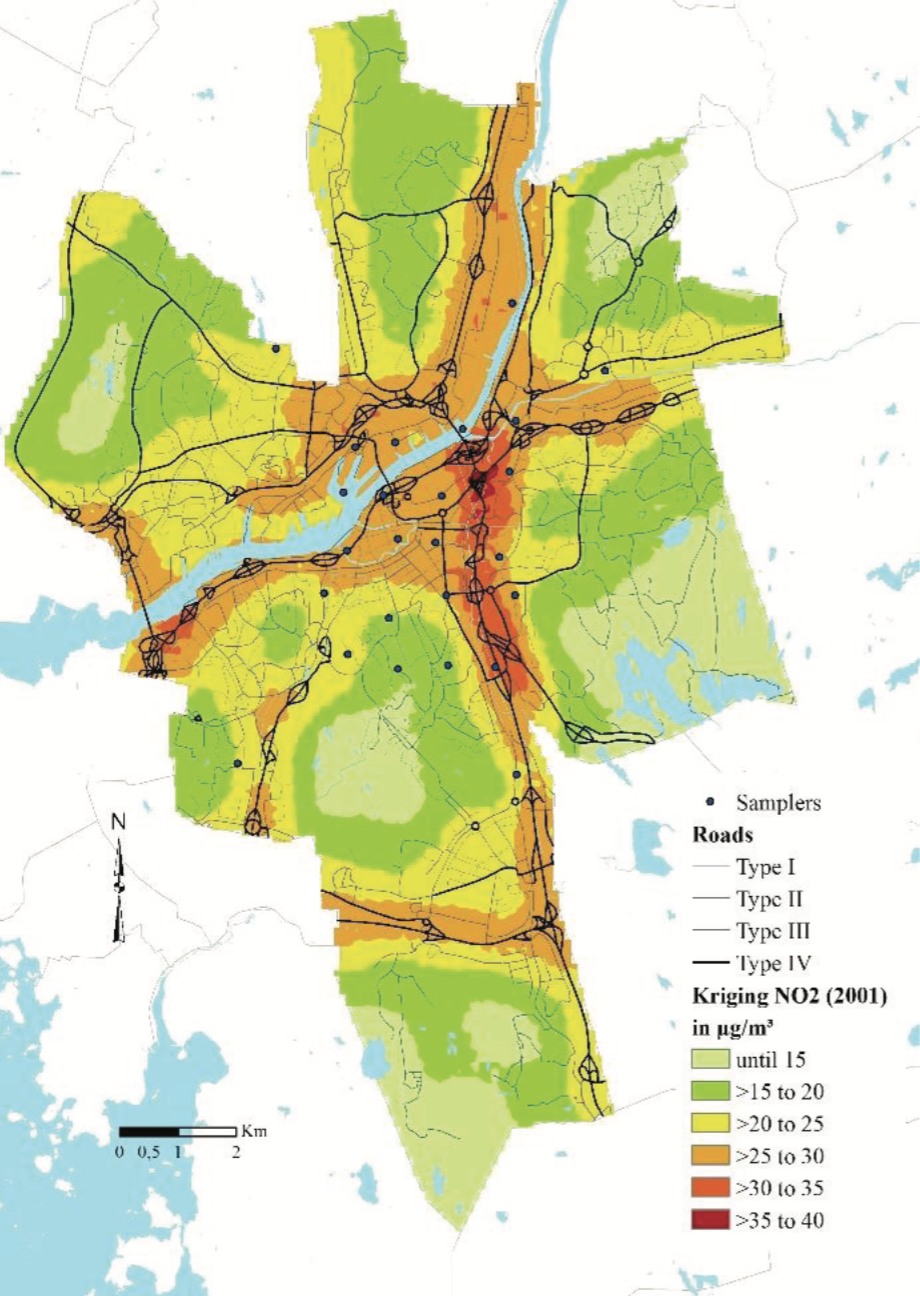
\includegraphics[height=8cm]{images/pollution_gothenburg.png}
    	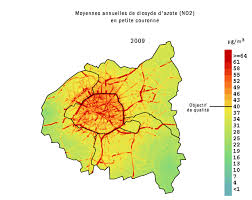
\includegraphics[height=8cm]{images/parisno2.jpg}
    \end{center}
    On constate que la pollution est phénomène spatial, et que le $NO_2$ est principalement concentré autour des grands axes routiers. Il est aussi pertinent de différencier les routes en différentes catégories selon leur fréquentation. Notons au passage que les routes sont classés selon différents types qui semblent être déterminants pour la pollution en $NO_2$, or nous n'avons qu'un type de route à notre disposition, et aucune information sur l'affluence. On peut donc sans aucun doute trouver des points qui auront les même valeurs statiques (surfaces cumulées) et pour lesquels le niveau de pollution est pourtant très différent.   
  \item
  	Si l'on cherche une carte de répartition de mircoparticules, on trouve ce type de données (source http://www.chroniques-cartographiques.fr) :
  	\begin{center}
  		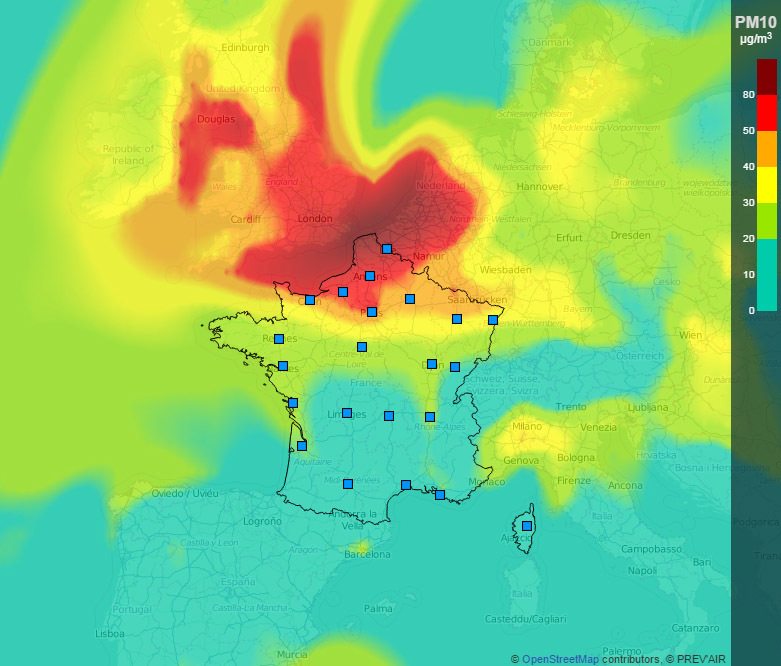
\includegraphics[width = 0.5\linewidth]{images/francepm10.jpg}
  	\end{center}    
  	Il apparaît donc que les mirco-particules se répartissent de façon nettement plus globales, et donc sont a priori beaucoup plus sensibles aux phénomènes météorologiques qu'aux données statiques, très locales.
  \item
    Nous avons fait un script pour vérifier autant que possible la cohérence des données, pour avoir une une idée du niveau de fiabilité des différents paramètres du problème. Nous avons alors repéré que l'angle d'orientation du vent nous est donnée par son cosinus et son sinus, dont la somme des carrés ne font pas 1 en général (moyenne = 0.995, écart type =  0.06 , maximum =  1.995 , minimum = 2.4 $\cdot 10^{-11}$)
 
    
\end{itemize}



\subsection{Exploration des valeurs}

\subsubsection{Influence des données constatées en première approche}
%Faire analyse de l'influence a posteriori, pca, ect...
%Pluie, vent ect..

\subsubsection{Les données dynamiques}

Pour se rendre compte de la répartition des valeurs des données dynamiques, on affiche les histogramme de ces valeurs sur une echelle logarithmique:

% 2 fois pression !
\begin{figure}[H]
	\captionsetup{labelformat=empty}
	\minipage{0.50\textwidth}
	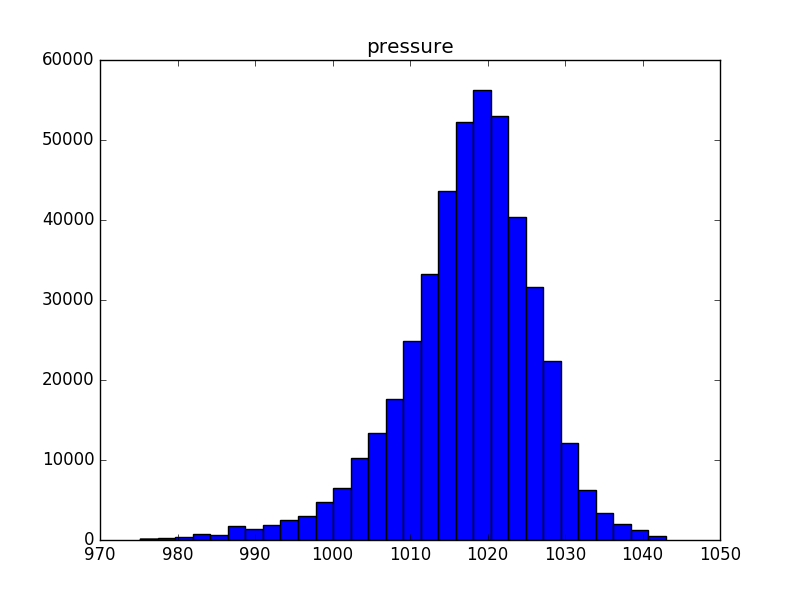
\includegraphics[width=\linewidth]{images/pression.png}
	\caption{pression}
	\endminipage\hfill
	\minipage{0.50\textwidth}
	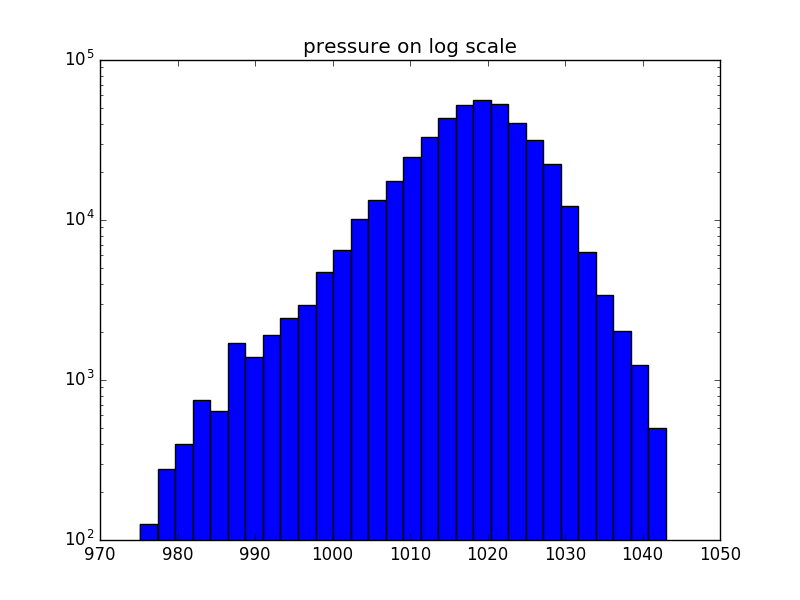
\includegraphics[width=\linewidth]{images/log_pression.png}
	\caption{pression sur échelle log}
	\endminipage\hfill
\end{figure}



Il apparaît donc que les données sont plus étalées sur un échelles logarithmique.
Dans la mesure ou nous cherchons à appliquer des techniques de régression simples %pourquoi ? expliquer !
et avec une forte régularité (regression lineaire), le fait d'utiliser des échelles logarithmiques est une première transformation que nous pouvons appliquer à nos données avant d'utiliser des modèles de régression simples.

\subsubsection{Les données statiques}

Les données statiques ne sont pas toutes renseignées sur certaines stations. Cela peut être problématique si l'on souhaite utiliser un algorithme d'apprentissage commun à toute les stations. Cependant, nous avons au moins une valeur par catégorie dans les données de type concentration cumulées, ce qui nous a permis d'interpoler les valeurs manquantes. Pour les autres (industrie, port, zones naturelles), les données sont considérées comme nulles si non renseignées, ce qui semble être raisonnable.


\subsection{Conclusion}

En conclusion, les données du problèmes sont peu fiables et discutables. Le fait que les données sur les routes ne soient pas différenciées sera surement un problème pour prédire les concentrations de $NO_2$. De même, partager les même données dynamiques pour toutes les stations d'une zone est discutable, surtout concernant la force et l'orientation du vent, jouant pourtant un rôle essentiel dans l'évolution de la concentration.

Un autre aspect important est cette distinction entre les données statiques (très variées et dont nous disposons que de 17 exemples) et les données dynamiques en grand nombre, identiques par zone, mais non redondantes entre les zones. Cela nous empêche donc d'apprendre un modèle par zone, et nuit à l'apprentissage d'un modèle commun aux zones. Cet aspect est la principale difficulté du problème.  

Nous pouvant ainsi dès à présent anticiper que les prévisions de ce problème resteront très grossières, surtout concernant le $NO_2$.



\section{Transformation des données}

\subsection{Les données dynamiques}

\subsubsection{Echelle}

Pour se rendre compte de la répartition des valeurs des données dynamiques, on affiche les histogramme de ces valeurs sur une echelle logarithmique:

\begin{figure}[H]
\captionsetup{labelformat=empty}
\minipage{0.50\textwidth}
  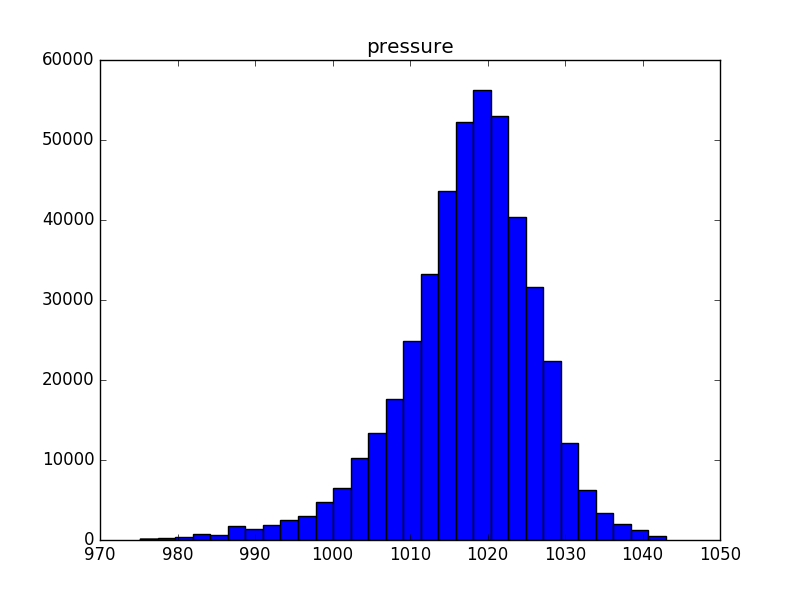
\includegraphics[width=\linewidth]{images/pression.png}
  \caption{pression}
\endminipage\hfill
\minipage{0.50\textwidth}
  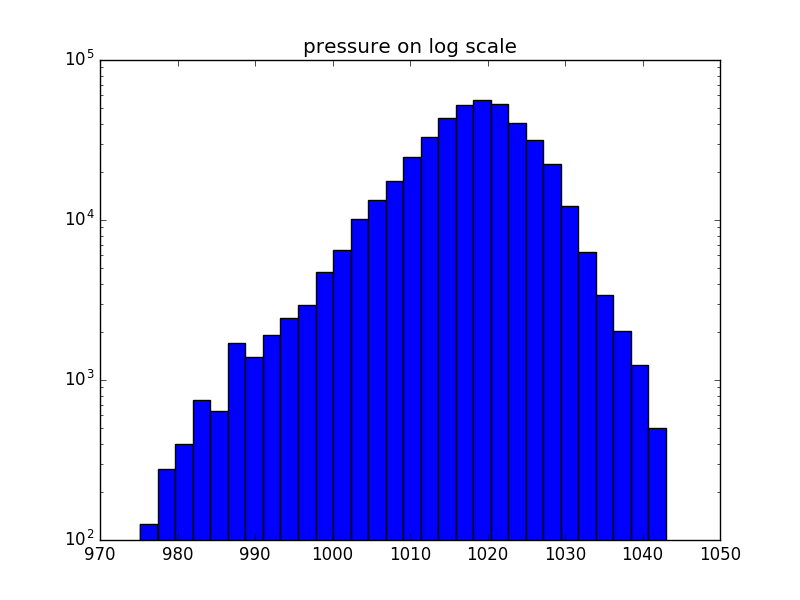
\includegraphics[width=\linewidth]{images/log_pression.png}
  \caption{pression sur échelle log}
\endminipage\hfill
\end{figure}

\begin{figure}[H]
\captionsetup{labelformat=empty}
\minipage{0.50\textwidth}
  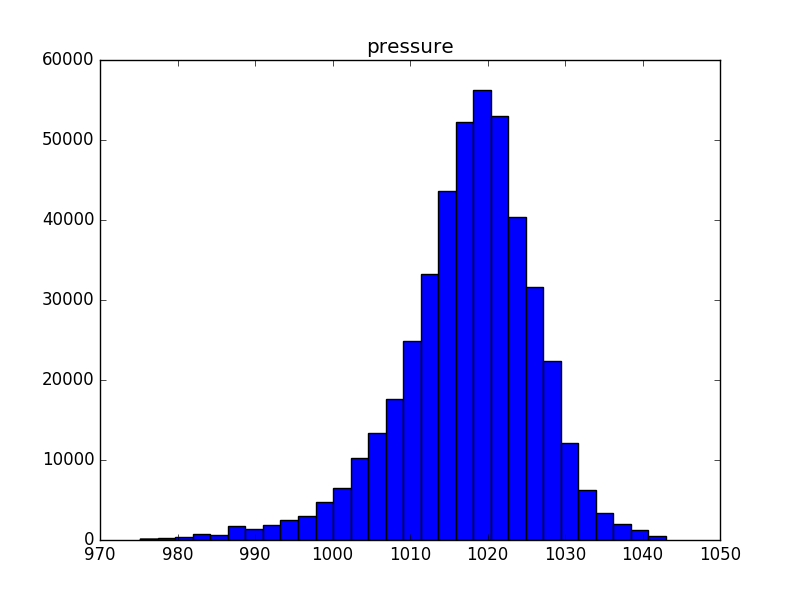
\includegraphics[width=\linewidth]{images/pression.png}
  \caption{pression}
\endminipage\hfill
\minipage{0.50\textwidth}
  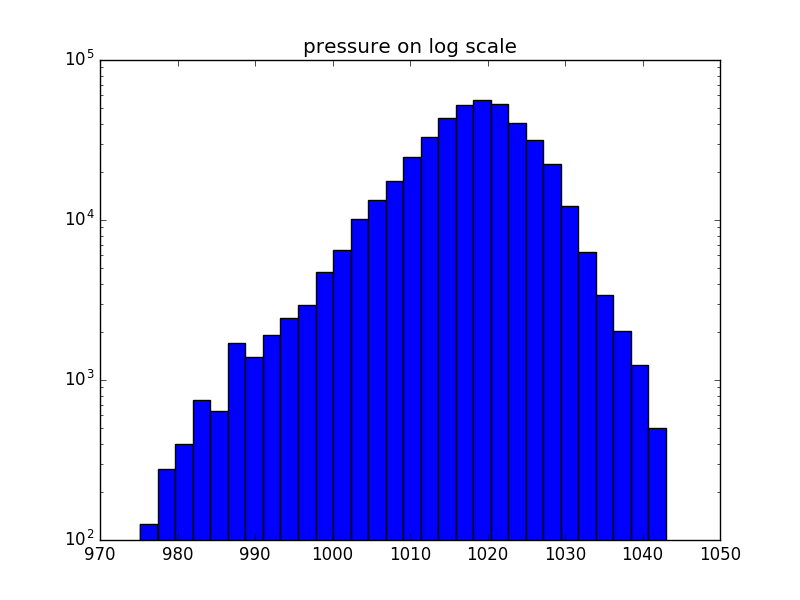
\includegraphics[width=\linewidth]{images/log_pression.png}
  \caption{pression sur échelle log}
\endminipage\hfill
\end{figure}

\begin{figure}[H]
\captionsetup{labelformat=empty}
\minipage{0.50\textwidth}
  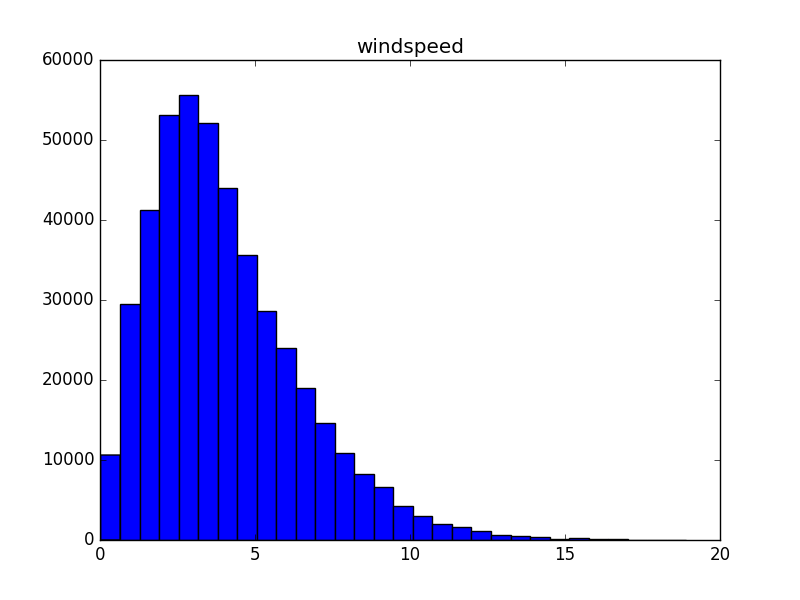
\includegraphics[width=\linewidth]{images/vent.png}
  \caption{vent}
\endminipage\hfill
\minipage{0.50\textwidth}
  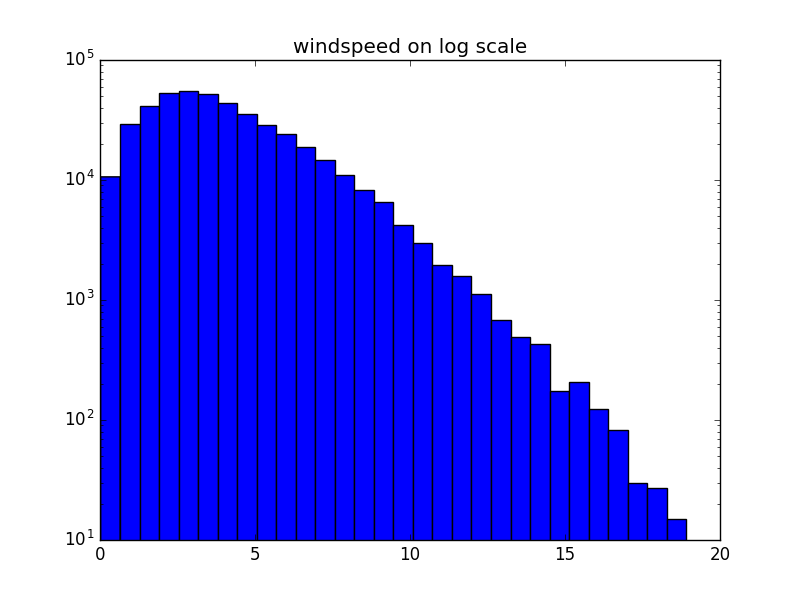
\includegraphics[width=\linewidth]{images/log_vent.png}
  \caption{vent sur échelle log}
\endminipage\hfill
\end{figure}

\begin{figure}[H]
\captionsetup{labelformat=empty}
\minipage{0.50\textwidth}
  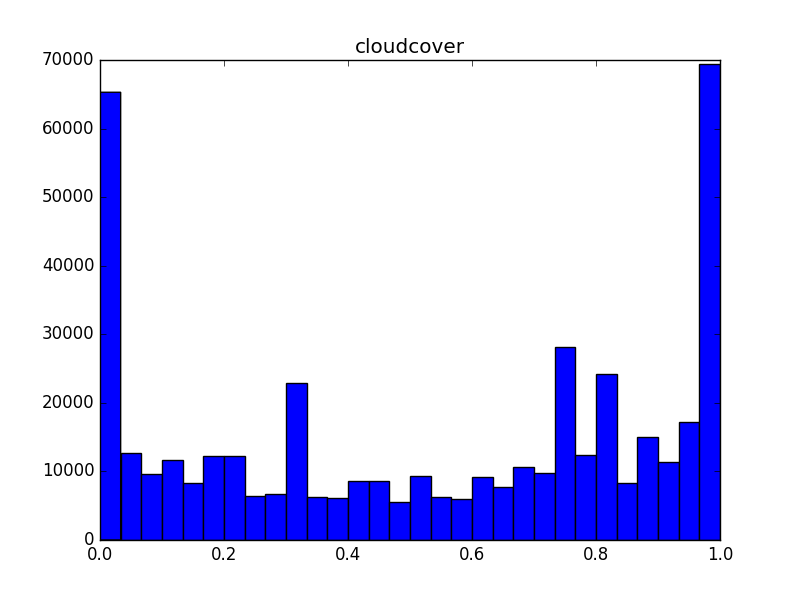
\includegraphics[width=\linewidth]{images/ennuagement.png}
  \caption{ennuagement}
\endminipage\hfill
\minipage{0.50\textwidth}
  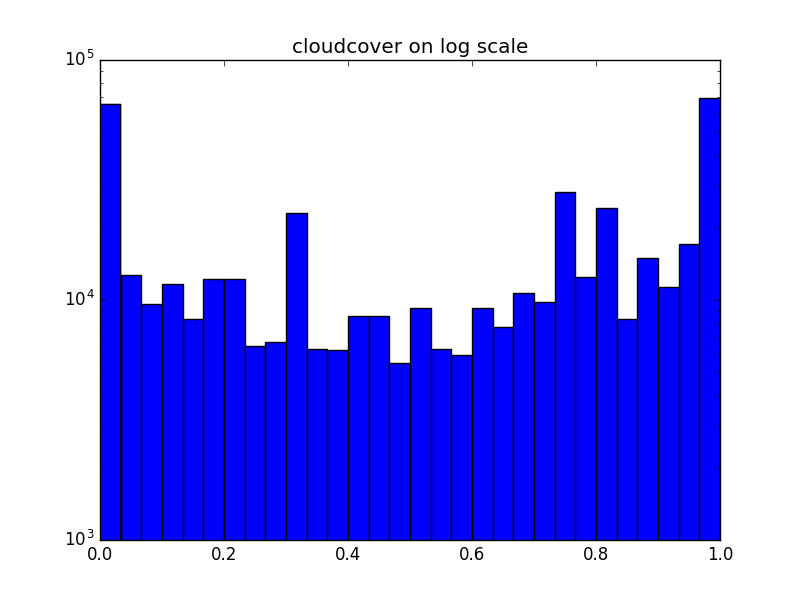
\includegraphics[width=\linewidth]{images/log_ennuagement.png}
  \caption{ennuagement sur échelle log}
\endminipage\hfill
\end{figure}

\begin{figure}[H]
\captionsetup{labelformat=empty}
\minipage{0.50\textwidth}
  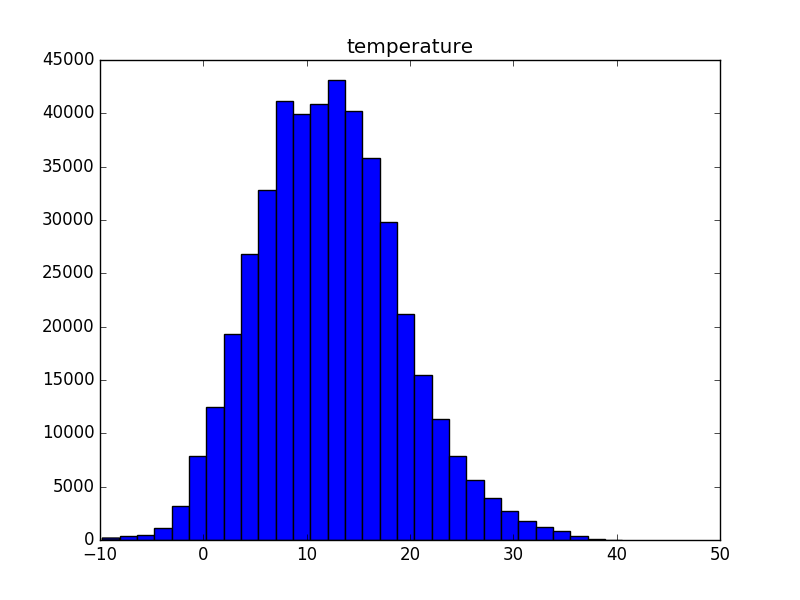
\includegraphics[width=\linewidth]{images/temperature.png}
  \caption{temperature}
\endminipage\hfill
\minipage{0.50\textwidth}
  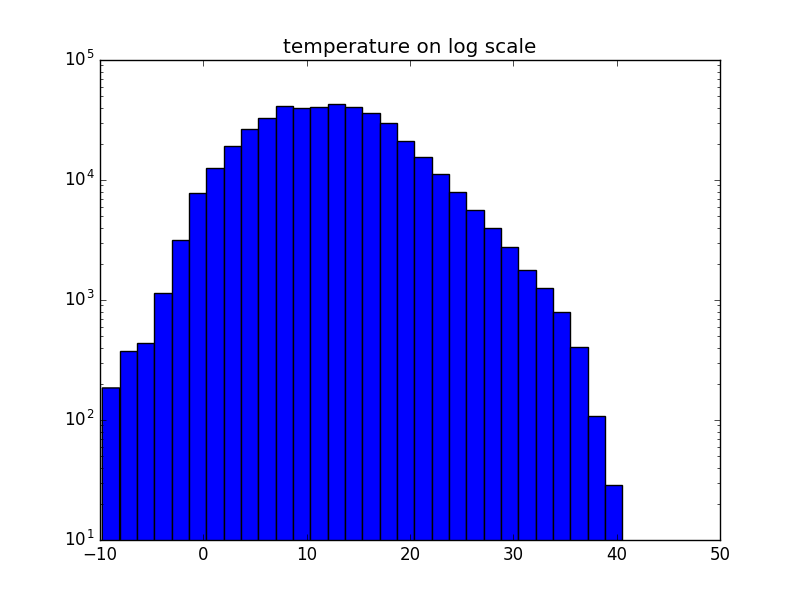
\includegraphics[width=\linewidth]{images/log_temperature.png}
  \caption{temperature sur échelle log}
\endminipage\hfill
\end{figure}

Il apparaît donc que les données sont plus étalées sur un échelles logarithmique.
Dans la mesure ou nous cherchons à appliques des techniques de régression simples et avec une forte régularité (regression lineaire), le fait d'utiliser des échelles logarithmiques est une première transformation que nous pouvons appliquer à nos données avant d'utiliser des modèles de régression simples.

\subsubsection{Représentations temps fréquence}

\subsection{Les données statiques}

Les données statiques sont des surfaces cumulées dans des périmètres de plus en plus grands



\section{Techniques existantes}

Dans la description du challenge, Plume Labs donne les références de deux articles qui décrivent et implémentent un modèle de régression de la pollution.
Le premier \cite{NO2reg} traite exclusivement le cas de la pollution en $NO_2$, qui est prédité uniquement à partir de variables statiques.
En effet, le $NO_2$ est nettement moins sensible aux précipitations que les particules.
Les données statiques utilisées pour la régression sont beaucoup plus précises que celles que nous avons à disposition:
\begin{itemize}
  \item 4 types de routes sont distingués
  \item on a les valeurs du traffic routier moyen dans des zones de différents rayons
  \item l'altitude est donnée
  \item les batiments sont classés par taille
\end{itemize}

La prédiction faite avec le modèle de régression est précise à 60\%, et la carte des prédictions est la suivante:

\begin{figure}
\begin{center}
  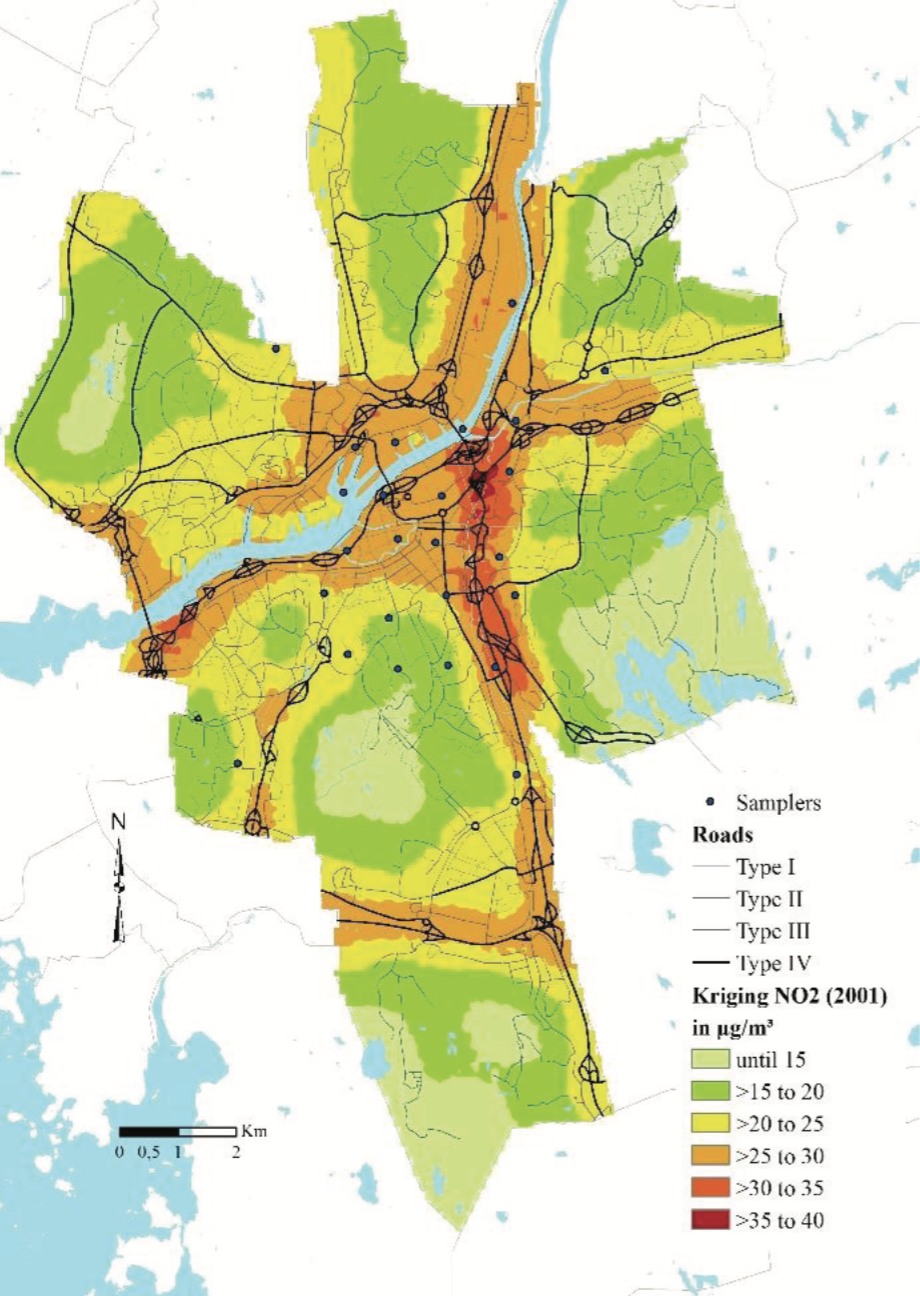
\includegraphics[height=9cm]{images/pollution_gothenburg.png}
  \caption{Carte des prédictions des concentration en $NO_2$ sur la ville de Gothenburg, source : \cite{NO2reg}}
\end{center}
\end{figure}

On voit par exemple que les différents types de routes ont une importance déterminante dans la prédiction de pollution.
Avec un seul type de route à disposition, les prédictions s'annoncent compliquées.

De plus, les données d'entrainement sont beaucoup plus conséquentes: pour une seule ville, il y a 24 points pour lequels la pollution est connue (points noirs sur la carte) et nous n'en avons que 3 par ville.


Le second article \cite{PMreg} traite exclusivement le cas des particules ultrafines (diamètre inférieur à 0.1 micromètres), auxquelles n'appartiennent pas les particules $PM_{10}$ et $PM_{2.5}$ que nous étudions.
Cette fois ci, les données sont constituées de données statiques et de données météorologique, et là encore, les données statiques sont beaucoup plus précises que celles que nous avons.
Les données d'entrainement proviennent de capteurs mobiles montés sur des vélos ou des voitures, ce qui permet d'avoir une sestimmation sur toute l'aire géographique, mais à des instants différents, représentés sur la carte suivante:

\begin{figure}
\begin{center}
  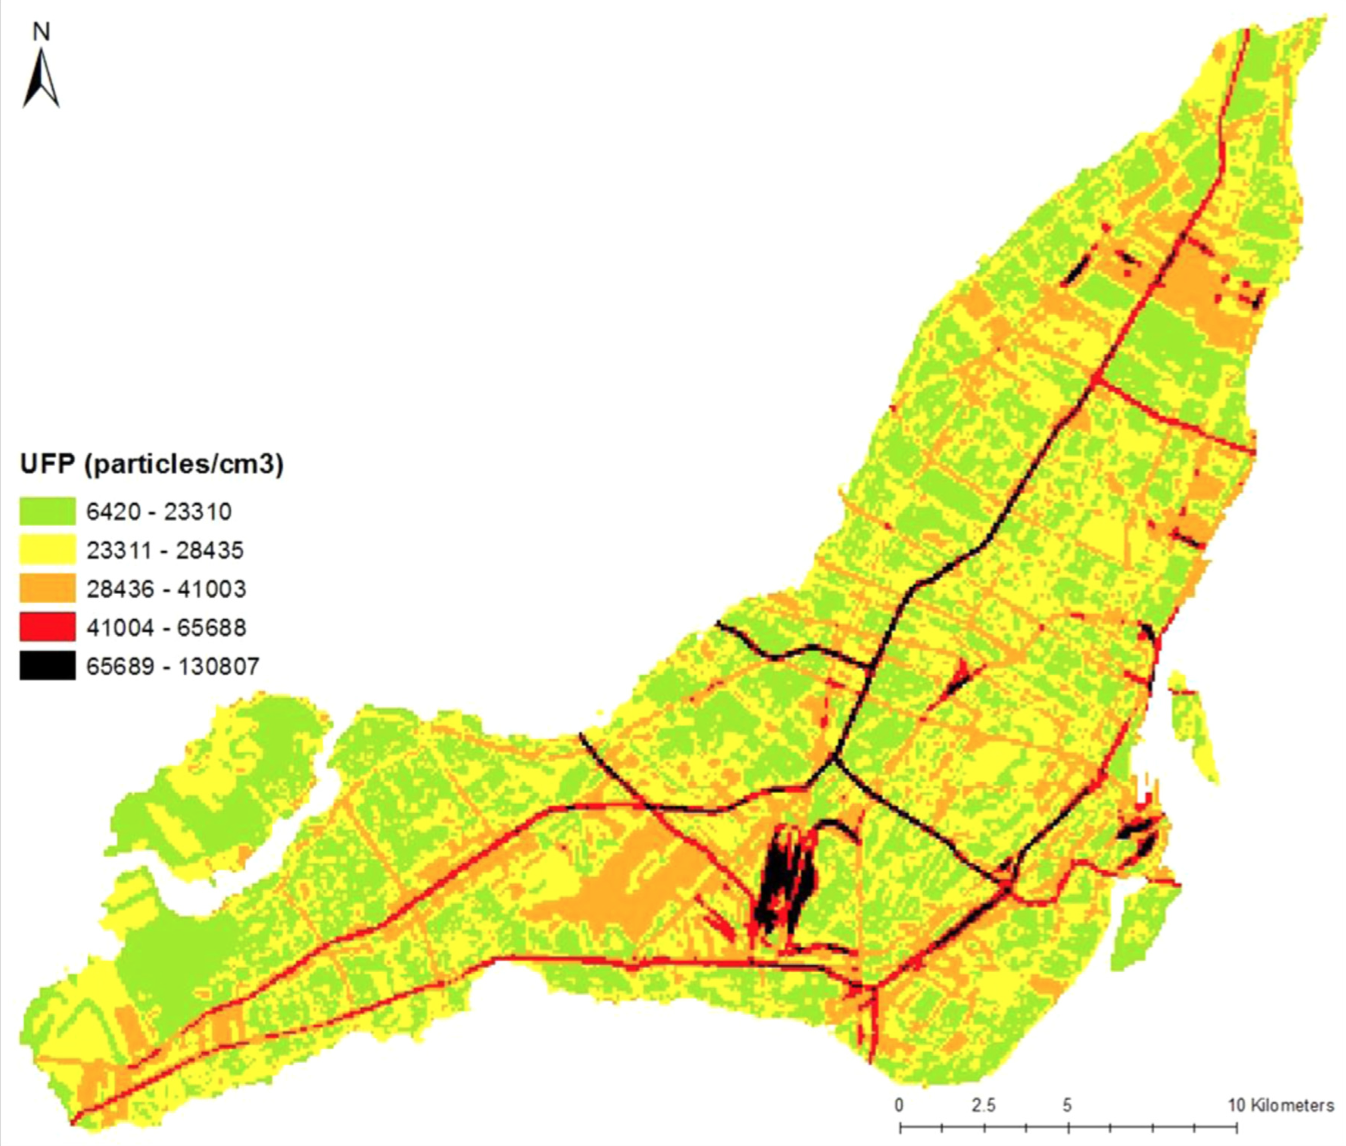
\includegraphics[height=9cm]{./images/pollution_montreal.png}
  \caption{Carte des mesures de particules sur la ville de Montréal, source : \cite{PMreg}}
\end{center}
\end{figure}

La prédictions atteint une précision de 79\%.
On retrouve le même genre de constat que pour le premier problème : les grands axes routiers sont d'une importance première.

La lecture de ces articles nous apprend que des techniques de régression basées sur des données statiques peuvent expliquer en grande partie la pollution (60\% à 80\%), mais les données nécessaires à de telles prédictions doivent être fines.


\section{Solutions}

Comme nous l'avons vu dans la section 1, le principal défi du problème est de réussir à traiter avec le bivalence des données. En outre, 

\subsection{Plus proche voisins}

On commence par implémenter une methode des K plus proches voisins sur les données brutes séparées polluant par polluant.
On fait plusieurs essais et voici ce qu'on obtient:

\begin{tabular}{|c|c|c|}
  \hline
  score & methode & K \\
  \hline
  597.379 &  par polluant & K = 5\\
  \hline
  617.229 & par polluant & K = 3\\
  \hline
  613.892 & par polluant  & K = 4\\
  \hline
  613.892 & par polluant et par zone & K = 4\\
  \hline
\end{tabular}

Etonnament, le fait de faire la méthode par polluant et par zone ne change pas le résultat.
De plus, on n'est pas très loin du score du benchmark proposé par Plume Labs (501).

\subsection{Méthode triviales}

On essaie ensuite trois méthodes triviales:
\begin{itemize}
  \item
    On met la valeur zéro pour toutes les prédictions: le score de 800 environ.
    Cela nous donne un ordre de grandeur sur les score: toute méthode donnant un score supérieur à 800 n'est vraiment pas adaptée.
  \item
    On met une valeur constante pour chaque polluant égale à la moyenne de toutes les valeurs pour ce polluant: on obtient une score de 380 environ.
  \item
    On calcule la valeur moyenne pour chaque polluant à chaque instant donné: on obtient un score de 440.000 environ.
    Cette méthode n'apporte rien par rapport à la valeur moyenne %A commenter
\end{itemize}

\subsection{Application brut aux données}

\subsubsection{Régression linéaire}

On teste un modèle linéaire sur les données.
Puisque le modèle linéaire contient les fonctions constantes, a priori, le score devrait être au pire de l'ordre de la valeur obtenue en mettant la moyenne, c'est à dire 350.000.
Etonnament, on obtient un score de 430.000.
Cela veut dire qu'avec une classe de fonction aussi simple que les fonctions linéaires, on overfitte déjà sur les données d'entrainement. Ou alors les données test réagissent différemment que les données d'entrainements, dû par exemple à un paramètre important manquant. 
Mais ce n'est pas tellement étonnant; en effet, nous n'avons que 29 jeu de données statiques alors que ces données vivent dans un espace de dimension 18.
Quelque soit la méthode employée, à moins d'avoir de la chance, on ne peut pas espérer obtenir une bonne prédiction. %A moderer ....

\subsubsection{Gradient boosting}

Nous avons choisi de tester également un algorithme plus élaboré et plus adapté au problème. Nous avons choisi la random forest (ou communement appelée gradient boosting dans sa version boostée, pour améliorer les performances et réduire l'overfitting). En effet, les types de données du problème sont très diverses (mesure physiques, boolean, probabilités, ...), et bien qu'étant une régression, ce problème à une valeur décisionnelle importante. Comme nous l'avons vu, de nombreux paramètres interviennent de façon binaires. Par exemple beaucoup de vent ou beaucoup de pluie va entrainer automatiquement peu de polluant. Enfin, comme expliqué, le risque d'overfitting est énorme.

Nous avons donc fait tourner un algorithme de gradient boosting sur les données, après avoir interpolé les valeurs statiques manquantes, et avoir numéroté les différents polluants.

Dans notre protocole, pour se rendre d'un éventuel overfitting, nous avons séparé les données d'entrainement en train/validation par station. Ainsi nous sommes a priori exactement dans les mêmes conditions que lors de la prédiction des données test. En outre, les données test ayant exactement les mêmes paramètres dynamiques par zone que les données d'entrainement, il est impossible de faire de l'overfitting vis-à-vis de ces-derniers.

Nous avons comme résultat : 261 sur les données de validation, 302 sur les données test.

Sur les données de validation, nous avons des prédictions nettement meilleurs sur les microparticules (environ 100) que sur le $NO_2$ (465), ce qui rejoint notre analyse a priori des données. En outre, nous pouvons afficher l'importance relative des données lors de l'apprentissage.

\begin{center}
	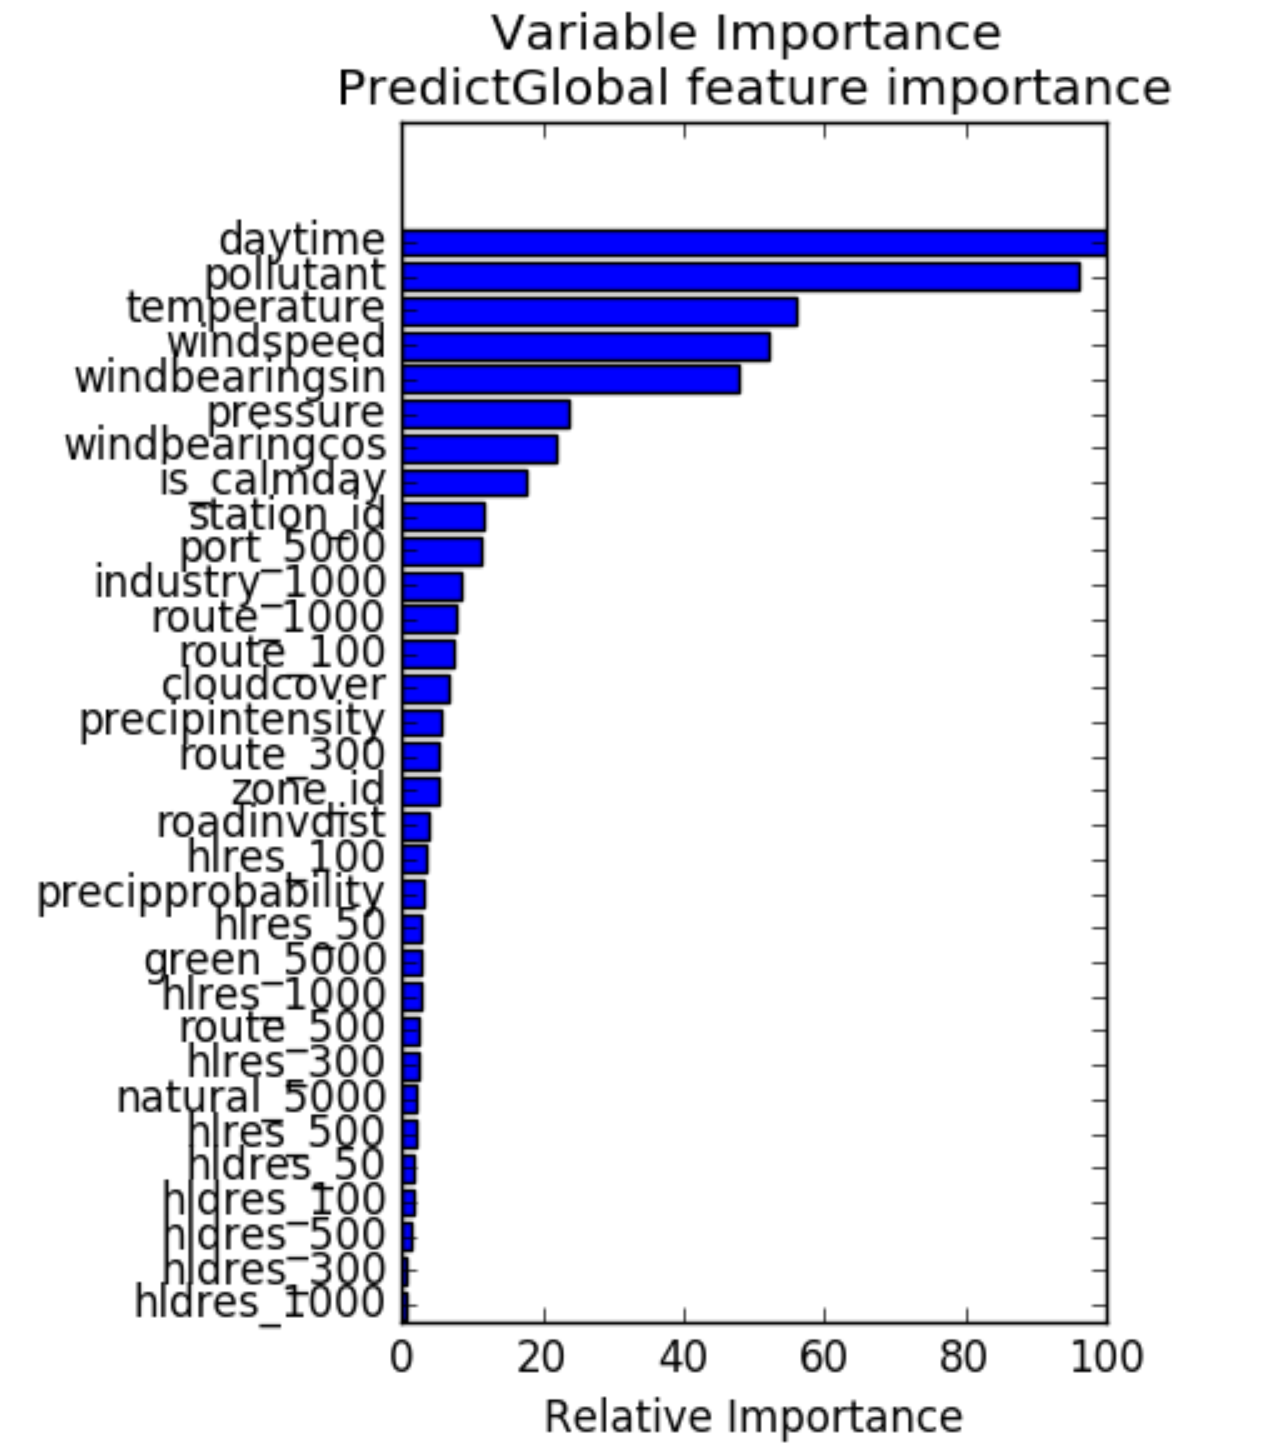
\includegraphics{images/importance feature global.png}
\end{center}

Ce graphique est très instructif, et on voit qu'il confirme nos raisonnements a priori sur les données. 
\begin{itemize}
	\item Le type de polluant a joué un rôle crucial dans la prédiction, ce qui nous confirme dans l'idée de séparer les polluants.
	\item Les données statiques ont rôle moindre par rapport aux données dynamique, ce qui est étonnant, surtout pour les routes qui devrait beaucoup influer sur le $NO_2$. Cela nous conforte dans l'idée que les paramètres statiques en notre possession sont peu pertinents.
	\item Le temps joue en rôle crucial également dans la prédiction. Bien que n'intervenant pas physiquement sur les polluant, il régit les activités humaines (et influe certain paramètres physiques), et donc la création de polluants.
	\item le numero de la station (stationid) joue en rôle important aussi, supérieur aux données statiques. %A commenter
\end{itemize} 


\subsection{Arrangement des données}

\subsubsection{Gradient boosting}

Comme prévu, l'algorithme de gradient boosting fonctionne mieux que la régression linéaire, et ses résultats nous encouragent encore plus à séparer les polluants. Nous avons donc appliqué l'algorithme précédent à chaque polluant indépendamment. 

En outre, appliquer tel quel l'algorithme aux données est améliorable.
\begin{itemize}
	\item Etant donné l'importance du temps, qui est brut sous sa forme présente, nous avons divisé en plusieurs heure/mois/jour %A completer
	\item 
\end{itemize}  

Les résultats sont bien meilleurs : 

%Afficher graphique feature importance


\subsubsection{Séparation}

Jusqu'ici nous n'avons pas encore palier 

\subsection{Conclusion}


bla bla bla c'est pourri

\end{document}
